\documentclass{standalone}

\ifstandalone
	\usepackage{amsmath}
	\usepackage{pgfplots}
\fi


\begin{document}
	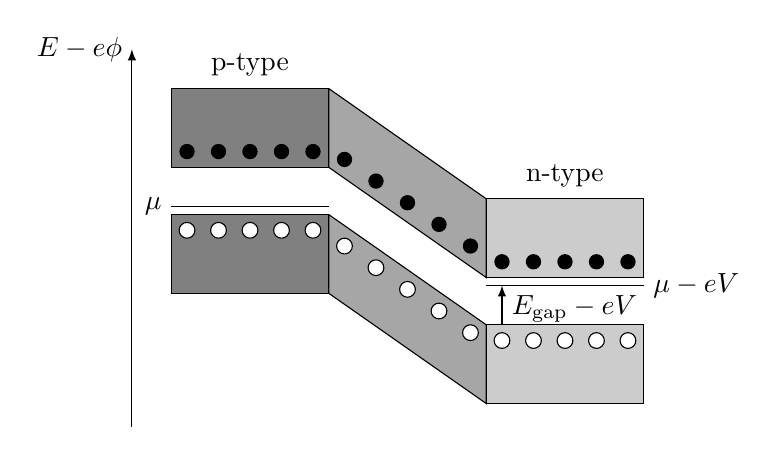
\begin{tikzpicture}
		\draw (1, 3.6) node {p-type};
		\draw (5, 2.2) node {n-type};
		\draw[-latex] (-0.5, -1) -- (-0.5, 3.8) node[left]{$E-e\phi$};
		\filldraw[draw=black, fill=gray] (0, 3.3) rectangle +(2, -1) +(0, -1.5) node[left]{$\mu$} -- +(2, -1.5) ++(0, -1.6) rectangle +(2, -1);
		\filldraw[draw=black, fill=gray!40] (4, 1.9) rectangle +(2, -1) +(0, -1.1) -- +(2, -1.1) node[right]{$\mu-eV$} ++(0, -1.6) rectangle +(2, -1);
		\filldraw[draw=black, fill=gray!70] (2, 3.3) -- ++(2, -1.4) -- ++(0, -1) -- ++(-2, 1.4) -- ++(0, 1);
		\filldraw[draw=black, fill=gray!70] (2, 1.7) -- ++(2, -1.4) -- ++(0, -1) -- ++(-2, 1.4) -- ++(0, 1);
		\draw[-latex] (4.2, 0.3) -- ++(0, 0.5);
		\draw (4.2, 0.5) node[right]{$E_\text{gap}-eV$};
		\foreach \x in {0, ..., 4} {
			\filldraw[fill=white] (0.2+0.4*\x, 1.5) circle (.10);
			\filldraw[fill=white] (2.2+0.4*\x, 1.3-0.275*\x) circle (.10);
			\filldraw[fill=white] (4.2+0.4*\x, 0.1) circle (.10);
			\filldraw[fill=black] (4.2+0.4*\x, 1.1) circle (.09);
			\filldraw[fill=black] (2.2+0.4*\x, 2.4-0.275*\x) circle (.09);
			\filldraw[fill=black] (0.2+0.4*\x, 2.5) circle (.09);
		};
	\end{tikzpicture}
\end{document}
